\section{Theoretische Grundlagen}
\label{sec:theoretGrundl}
Dieses Kapitel behandelt die theoretischen Grundlagen für verwendete Verfahren, Hardware und Software. Es hat die Aufgabe den Leser:innen für das Verständnis essentielle Informationen zu übermitteln.
\subsection{Globales Positionsbestimmungssystem}
\label{subsec:tGPS}
Das \ac{GPS} ist ein gängiges Navigationssystem, um die geografische Position zu ermitteln. Ursprünglich wurde \ac{GPS} für militärische Zwecke entwickelt und wird heutzutage vom Verteidigungsministerium der USA betrieben.\\
\ac{GPS} ist satellitengestützt und umfasst eine Anzahl von 32 Satelliten in der Erdumlaufbahn, wovon mindestens vier eine Verbindung mit dem GPS-Empfängermodul haben müssen, um die Position bestimmen zu können. Drei dieser Satelliten sind für die Erfassung der Längen- und Breitengrade, sowie die der Höhe notwendig, die Verbindung mit einem vierten Satelliten ermöglicht die Synchronisation der Uhr des Empfängers, mit der der Satelliten. Dies ist besonders ausschlaggebend, da nur bei einer exakten Übereinstimmung der Zeiten, die Position korrekt berechnet werden kann. Um die Position zu berechnen, wird die Zeit gemessen, die das Signal vom Satelliten zum Empfänger benötigt und in eine Distanz umgerechnet. Mithilfe der Entfernungen zu mehreren Satelliten vom Empfänger, kann über Triangulation die geografische Lage auf der Erdoberfläche ermittelt werden.\\
Die Genauigkeit der Positionserfassung variiert zwischen 13 Meter und 1 Millimeter. Abweichungen unter einem Meter sind allerdings fast nur mit professioneller, beziehungsweise militärischer Ausrüstung erreichbar. Mit Komponenten aus den Hobby-Elektronikbereich sowie in Smartphones, sind Genauigkeiten zwischen 13 und 3 Metern realistisch möglich.\\
Die Daten werden standardisiert im \ac{NMEA}-Format über eine serielle Schnittstelle ausgegeben. (\cite{schnabelGPS})


\subsection{Inertiale Messeinheit}
\label{subsec:tIMU}
Eine \ac{IMU} z. Dt. inertiale Messeinheit kombiniert mehrere verschiedene Sensoren zur Bestimmung von Lage, Beschleunigungen und Position im dreidimensionalen Raum. Um eine zuverlässige Ermittlung dieser Werte zu gewährleisten, werden Beschleunigungsmessung, Rotationsgeschwindigkeitsmessung (und in einigen Fällen auch die Messung des Magnetfeldes der Erde) kombiniert. Inertiale Messeinheiten werden unter anderem für die Navigation von Flugzeugen, Raumschiffen und Schiffen verwendet. In der Automobilindustrie werden \ac{IMU}s verwendet, um das Fahrverhalten von Autos zu bestimmen und dieses zu verbessern.\\
Die \ac{IMU} liefert die Beschleunigungen sowohl in x-, y- als auch z-Richtung, die Winkelgeschwindigkeiten um die x-, y- als auch z-Achse (und in manchen Fällen die magnetische Feldstärke in x-, y- als auch z-Richtung). Um die Lage zu bestimmen können die Beschleunigungssensoren verwendet werden, indem die Lage der Erdbeschleunigung im dreidimensionalen Raum ermittelt wird, dies funktioniert allerdings nur, solange der Sensor sich in Ruhelage befindet. Alternativ können die Rotationsgeschwindigkeiten integriert werden, dies ergibt aber aufgrund von Messfehlern nach einiger Zeit Abweichungen (drift).\\ Um eine fehlerfreie Ermittlung der Lage zu ermöglichen kann Sensorfusion betrieben werden. Darunter versteht man einen Prozess, der Signale von zwei oder mehr Sensoren zusammenfasst. Im Falle einer \ac{IMU} kann die Ermittlung mittels Accelerometern, Gyroskopen und Magnetometern wie in Sektion \ref{subsec:IMUprogram} beschrieben kombiniert werden.
(\cite{UCAM-CL-TR-696})

\subsection{Hall-Effekt}
\label{subsec:tHall}

\subsection{Infrarot-Lichtschranke}
\label{subsec:tIR}

\subsection{Raspberry Pi Zero 2 W}
\label{subsec:RasPi}
Der Raspberry Pi Zero 2 W ist ein Einplatinencomputer der Raspberry Pi Foundation. Mit einem 1GHz quad-core 64-bit Arm Prozessor, 512MB SDRAM, eingebauten WLAN- und Bluetooth-Modulen und 40 pins für GPIO, SPI, I2C, UART und Spannungsversorgung stellt er ein Umfangreiches Paket für die Interaktion mit diverser Sensorik dar. Als Betriebssystem bietet die Raspberry Pi Foundation eine auf Debian basierte Linux-Distribution namens Raspberry Pi OS an. Raspberry Pi OS ist in drei verschiedenen Varianten verfügbar, diese unterscheiden sich im Funktionsumfang und der Installationsgröße. Aufgrund der limitierten Rechenleistung des \ac{Raspi} Zero 2 W und der fehlenden Notwendigkeit für eine Desktop-Umgebung ist die Lite-Version am besten geeignet.
\begin{figure}[h]
\centering
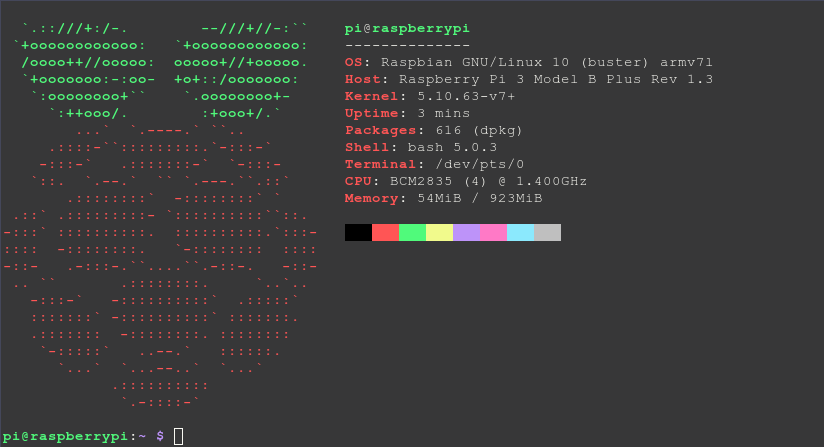
\includegraphics[scale=0.6]{pineofetch.png}
\caption{Das Commandline-Tool neofetch am \ac{Raspi} Zero 2 W}
\label{fig:pineofetch}
\end{figure}

\subsection{Python}
\label{subsec:tPython}
Python ist eine in den frühen 1990ern von Guido van Rossum erstellte Programmiersprache. Heutzutage zeichnet sich Python dadurch aus, dass es quelloffen und für jeden nutzbar ist. Außerdem nimmt Python dem Programmierenden durch die im Vergleich zu Sprachen wie C++ einfache Syntax und das integrierte Ressourcenmanagement viel Arbeit ab. Ein Nachteil von Python ist, dass es im Vergleich mit anderen Sprache wie C++ eine sehr langsame Programmiersprache ist. Aufgrund seiner Simplizität und Verfügbarkeit für Plattformen wie Microsoft Windows, macOS, Linux und FreeBSD gibt es sehr viele quelloffene Bibliotheken für Python, was das Programmieren noch weiter erleichtert. Ein weiterer Unterschied zu Sprachen wie C, C++ oder Rust besteht darin, dass Python interpretiert statt kompiliert wird. Dies hat zur Folge, dass der Code direkt ausgeführt werden kann, solange ein geeigneter Python-Interpreter und die verwendeten Bibliotheken installiert sind, ohne zuvor für jede Plattform eigens kompiliert werden zu müssen.
(\cite{matthes-2019})

\subsection{Qt}
\label{subsec:tQt}
Qt ist eine von der Qt Company entwickelte Bibliothek für die Entwicklung von grafischen Oberflächen. Sie ist wie Python plattformübergreifend und unterstützt unter anderem Microsoft Windows, macOS, Unixartige Betriebssysteme mit X11, Linux mit Wayland, Android und iOS. Qt unterstützt ebenfalls die Entwicklung mit verschiedenen Programmiersprachen, darunter Python, C++ und Qt QML, zusätzlich wird Unterstützung für Rust und Go von der Qt-Community angeboten. Qt ist wie Python Quelloffen und kann für die Open-Source-Programmierung frei verwendet werden. Die neueste Qt-Python Bibliothek heißt PySide6, mit nur fünf Zeilen Python-Code kann ein leeres Fenster erstellt werden.
\begin{figure}[h]
\centering
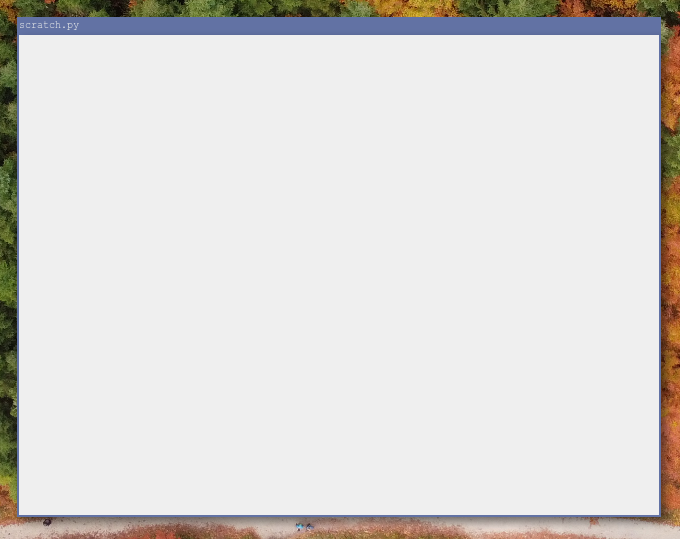
\includegraphics[scale=0.5]{EmptyQtWindow.png}
\caption{Leeres PySide6-Fenster auf Linux unter X11}
\label{fig:EmptyQtWindow}
\end{figure}

\subsection{FDM-3D-Druck}
\label{subsec:tFDM}
\ac{FDM} z. Dt. Schmelzschichtung, ist eine gängige Methode der additiven Fertigung, die auch die Funktionsweise der meisten 3D-Drucker darstellt. Additive Fertigung bedeutet, dass ein zu herstellendes 3D-Modell in einzelnen Schichten mit der gewünschten Schichthöhe auf einer Plattform aufgetragen wird. Der Vorteil ist, die Möglichkeit komplexe Modelle zu fertigen, die mit herkömmlichen Fertigungsverfahren sehr schwer, oder gar unmöglich sind.\\
Bei der \ac{FDM}-Technologie wird ein Kunststoffdraht (Filament) durch eine erhitzte Düse gepresst, wodurch der Kunststoff geschmolzen und je nach Durchmesser der Düsenöffnung, in einem bestimmten Durchmesser extrudiert wird. Bei der \ac{FDM}-Methode können also ausschließlich Thermoplaste als Druckmaterial verwendet werden. Die Düse wird während dem Extrudier-Vorgang in einer bestimmten Höhe über einer (meist beheizten) Plattform, dem sogenannten Druckbett, bewegt, um die erste Schicht des Modells aufzutragen. Anschließend wird die Düse eine Schichthöhe angehoben, um die nächste Schicht auf der ersten aufzutragen (Siehe Abbildung \ref{fig:FDM}). Typische Schichthöhen von \ac{FDM}-Druckern sind 0,1 bis 0,4 Millimeter und die Düse hat meist einen Durchmesser von 0,4 Millimeter. Zu den möglichen Materialien zählen unter anderem \ac{PLA}, \ac{ABS}, \ac{PETG} sowie Nylon. Auch flexible Materialien sind möglich, welche meist mit erhöhten Drucker-Anforderungen verbunden sind. Bei Hobby-Druckern beträgt die typische maximale Druckgröße zwischen 120*120*120 und 300*300*300 Millimeter in x-, y-, und z-Richtung. Der große Nachteil von \ac{FDM} ist die Oberflächenbeschaffenheit des fertigen Bauteils, welche markante Rillen der einzelnen Schichten aufweist. (\cite{alexandreFDM})
\begin{figure}[h]
\centering
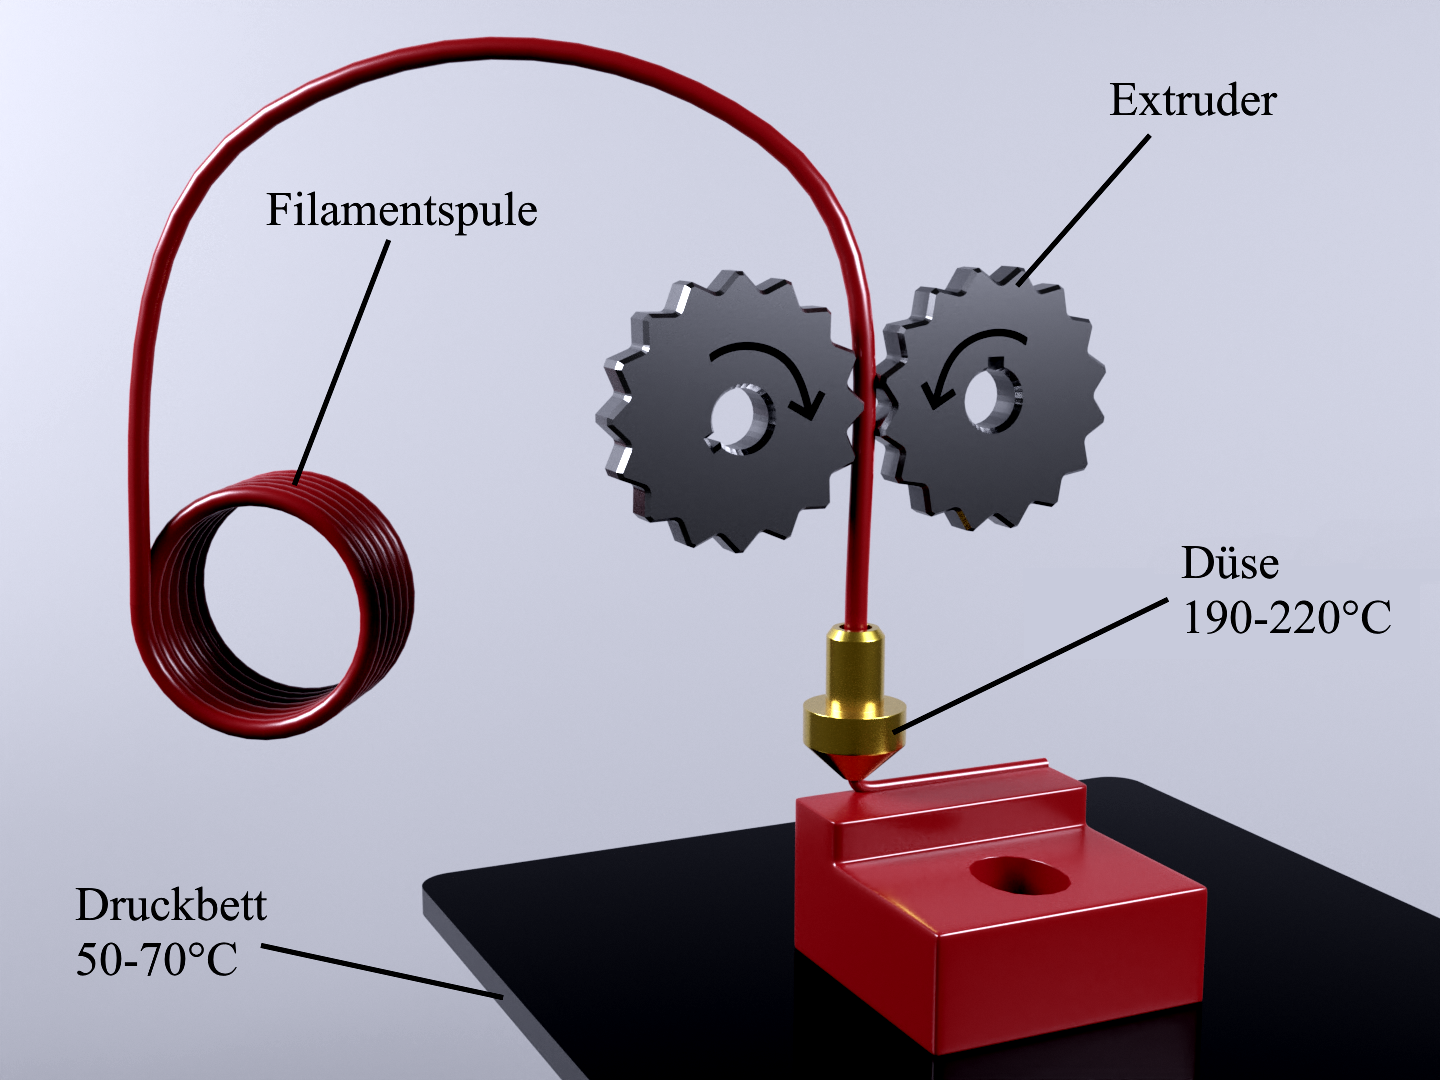
\includegraphics[scale=0.2]{FDM.png}
\caption{FDM-Funktionsweise}
\label{fig:FDM}
\end{figure}

\subsection{SLA-3D-Druck}
\label{subsec:tSLA}